\documentclass{article}
\usepackage[T1]{fontenc} 
\usepackage[utf8]{inputenc}
\usepackage{graphicx}
\usepackage{float}
\usepackage[czech]{babel}
\usepackage{rotating}

\begin{document}

\begin{titlepage}
    \begin{center}
        
\includegraphics[scale=0.1,keepaspectratio]{fig/logo_cz.png}
        
        \vspace{3cm}
        
        {\Huge Úvod do softwarového inženýrství}
        
        \vspace{0.25cm}
        
        {\LARGE 2019/2020}
        
        \vspace{2cm}
        
        {\LARGE Projekt IUS - Model informačního systému}
        
        \vspace{0.25cm}
        
        {\textbf{\LARGE Zadání č. 64 - Mafie}}
        \vfill
    \end{center}
    {\LARGE Karel Norek, xnorek01 \hfill \today}

\end{titlepage}

\textbf{\flushleft \LARGE 64. Mafie}

\vspace{0.25cm}

\large Padrino Guiseppe, přítel všech brněnských mafiánů, Vás požádal o vytvoření informačního systému pro organizaci kriminální činnosti a setkání předních brněnských rodin. 
\par V čele každé rodiny je Don (např. Don Calzone, Don Quatro Formagi, Don Funghi, apod.), respektovaná osoba, která organizuje dění rodiny, určena běžnými atributy (jméno, věk, velikost bot, ???). 
\par Samotná famílie pak sestává z řadových členů, kteří nemusí být pokrevně spřízněni a kteří zprostředkovávají veškerou kriminální činnost, jako je odstraňování nevhodných osob, dealování drog, tisknutí falešných peněz, atd., Don si však nikdy nešpiní ruce. 
\par Kriminální činnost probíhá v rámci území, určených gps souřadnicemi, adresou, rozlohou, a mohou být buď řádným rajónem jedné z familií, nebo neutrálním územím, kde může operovat větší počet familií. 
\par Do samotné kriminální činnosti jsou pak zapojeni konkrétní řadoví členové v různých obdobích (tzn. řadový člen může nejprve dealovat drogy a poté přejít na odstraňování osob), přičemž každá činnost je přímo vedena jednou z familií a má různou dobu trvání a tato operace má vždy unikátní jméno. 
\par Do těchto činností může být zapojeno více rodin, to v případě, že dvě rodiny uzavřou alianci, které však nemusí mít dlouhé trvání. 
\par Jednou z hlavních činností jsou pak vraždy, u kterých je vedeno nejen, kde byly provedeny, ale i kdo je provedl a na kom je provedl. Některé z těchto vražd jsou pak objednány samotnými Dony, jiné jsou spontánní, bez bližší objednávky. Cílem vraždy však nikdy není Don. 
\par Systém pravidelně organizuje setkání Donů, kde se probírají výsledky jednotlivých rodin a probíhají buď v rámci neutrálního území, nebo jsou hostěny některou z předních rodin. Systém pak zasílá Donům pozvánky a očekává od nich potvrzení účasti.

\newpage

\begin{figure}[H]
    \centering
    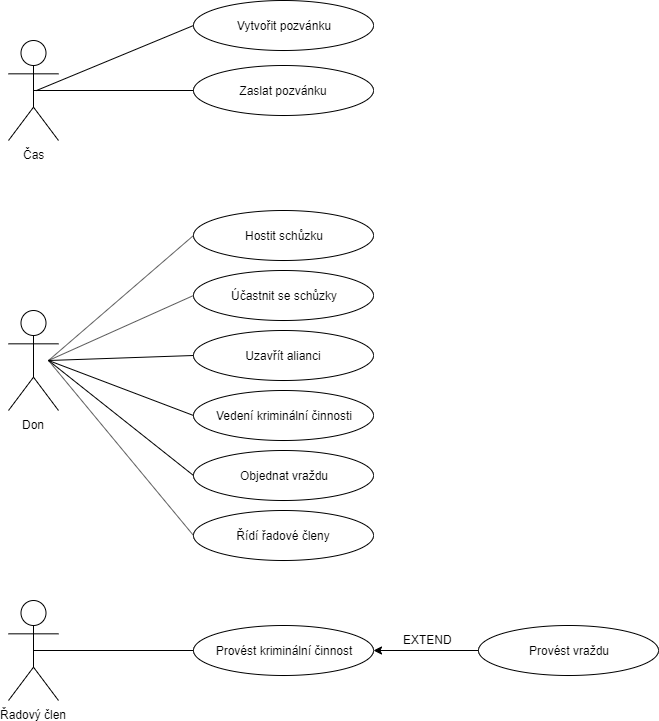
\includegraphics[scale=0.55, keepaspectratio]{fig/USCD.png}
    \caption{Use case diagram pro mafii}
    \label{fig:UCD}
\end{figure}

\newpage

\begin{sidewaysfigure}
    \centering
    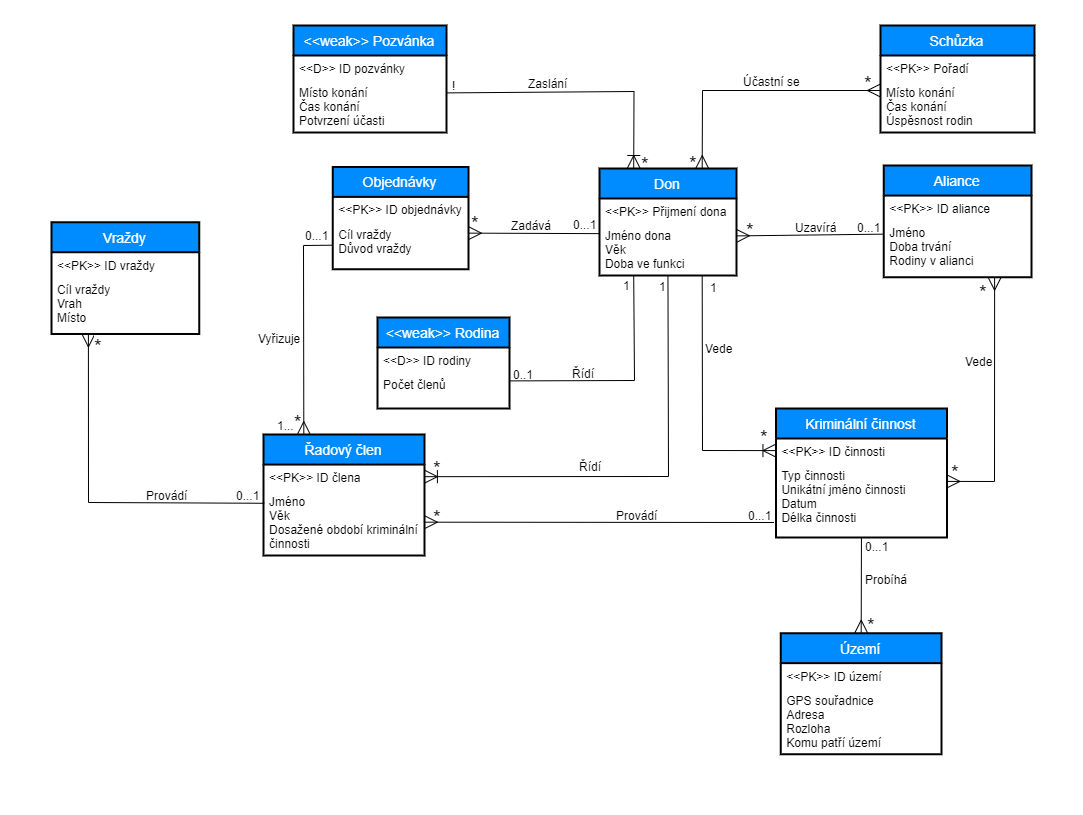
\includegraphics[scale=0.63, keepaspectratio]{fig/ERD.png}
    \caption{ER diagram pro mafii}
    \label{fig:ERD}
\end{sidewaysfigure}
    

\end{document}
